%%%%%%%%%%%%%%%%%%%%%%%%%%%%%%%%%%%%%%%%%%{{{
% Structured General Purpose Assignment
% LaTeX Template
%
% This template has been downloaded from:
% http://www.latextemplates.com
%
% Original author:
% Ted Pavlic (http://www.tedpavlic.com)
%
% Note:
% The \lipsum[#] commands throughout this template generate dummy text
% to fill the template out. These commands should all be removed when 
% writing assignment content.
%
%%%%%%%%%%%%%%%%%%%%%%%%%%%%%%%%%%%%%%%%%

%----------------------------------------------------------------------------------------
%	PACKAGES AND OTHER DOCUMENT CONFIGURATIONS
%----------------------------------------------------------------------------------------

\documentclass[12pt,a4paper]{article}

\usepackage{fancyhdr} % Required for custom headers
\usepackage[utf8]{inputenc}
\usepackage[french]{babel}
\usepackage{hyperref}
\usepackage{hyperref}
\usepackage{float}
\usepackage{lastpage} % Required to determine the last page for the footer
\usepackage{extramarks} % Required for headers and footers
\usepackage{graphicx} % Required to insert images
\usepackage{lipsum} % Used for inserting dummy 'Lorem ipsum' text into the template

% Margins
\topmargin=-0.45in
\evensidemargin=0in
\oddsidemargin=0in
\textwidth=6.5in
\textheight=9.0in
\headsep=0.25in 

\linespread{1.1} % Line spacing

% Set up the header and footer
\pagestyle{fancy}
\lhead{\hmwkAuthorName \ \hmwkTitle} % Top left header
\rhead{\firstxmark} % Top right header
\lfoot{\lastxmark} % Bottom left footer
\cfoot{} % Bottom center footer
\rfoot{Page\ \thepage\ de\ \pageref{LastPage}} % Bottom right footer
\renewcommand\headrulewidth{0.4pt} % Size of the header rule

\renewcommand\footrulewidth{0.4pt} % Size of the footer rule

\setlength\parindent{0pt} % Removes all indentation from paragraphs

%----------------------------------------------------------------------------------------
%	DOCUMENT STRUCTURE COMMANDS
%	Skip this unless you know what you're doing
%----------------------------------------------------------------------------------------

% Header and footer for when a page split occurs within a problem environment
\newcommand{\enterProblemHeader}[1]{
\nobreak\extramarks{#1}{#1 continue \ldots}\nobreak
\nobreak\extramarks{#1 (suite)}{#1 continue \ldots}\nobreak
}

% Header and footer for when a page split occurs between problem environments
\newcommand{\exitProblemHeader}[1]{
\nobreak\extramarks{#1 (continued)}{#1 continued on next page\ldots}\nobreak
\nobreak\extramarks{#1}{}\nobreak
}

\setcounter{secnumdepth}{0} % Removes default section numbers
\newcounter{homeworkProblemCounter} % Creates a counter to keep track of the number of problems
\newcounter{homeworkQuestionCounter} % Creates a counter to keep track of the number of problems

\newcommand{\homeworkProblemName}{}
\newenvironment{homeworkProblem}[1][Problem \arabic{homeworkProblemCounter}]{ % Makes a new environment called homeworkProblem which takes 1 argument (custom name) but the default is "Problem #"
\stepcounter{homeworkProblemCounter} % Increase counter for number of problems
\renewcommand{\homeworkProblemName}{#1} % Assign \homeworkProblemName the name of the problem
\section{\homeworkProblemName} % Make a section in the document with the custom problem count
\enterProblemHeader{\homeworkProblemName} % Header and footer within the environment
}{
\exitProblemHeader{\homeworkProblemName} % Header and footer after the environment
\setcounter{homeworkQuestionCounter}{0} % Removes default section numbers
}

\newcommand{\problemAnswer}[1]{ % Defines the problem answer command with the content as the only argument
\noindent\framebox[\columnwidth][c]{\begin{minipage}{0.98\columnwidth}#1\end{minipage}} % Makes the box around the problem answer and puts the content inside
}

\newcommand{\homeworkSectionName}{}
\newenvironment{homeworkSection}[1]{ % New environment for sections within homework problems, takes 1 argument - the name of the section
\stepcounter{homeworkQuestionCounter} % Increase counter for number of problems
\renewcommand{\homeworkSectionName}{\arabic{homeworkProblemCounter} . \arabic{homeworkQuestionCounter} #1} % Assign \homeworkSectionName to the name of the section from the environment argument
\subsection{\homeworkSectionName} % Make a subsection with the custom name of the subsection
\enterProblemHeader{\homeworkProblemName\ [\homeworkSectionName]} % Header and footer within the environment
}{
\enterProblemHeader{\homeworkProblemName} % Header and footer after the environment
}
   
%----------------------------------------------------------------------------------------
%	NAME AND CLASS SECTION
%----------------------------------------------------------------------------------------

\newcommand{\hmwkTitle}{TP1} % Assignment title
\newcommand{\hmwkDueDate}{Mardi\ 2 Février\ 2016} % Due date
\newcommand{\hmwkClass}{INF6422} % Course/class
\newcommand{\hmwkClassTime}{12h} % Class/lecture time
\newcommand{\hmwkClassInstructor}{François Labrèche} % Teacher/lecturer
\newcommand{\hmwkAuthorName}{Philippe Troclet (1815208) et Alexandre Mao (1813566)} % Your name

%----------------------------------------------------------------------------------------
%	TITLE PAGE
%----------------------------------------------------------------------------------------

\title{
\vspace{2in}
\textmd{\textbf{\hmwkClass:\ \hmwkTitle}}\\
\normalsize\vspace{0.1in}\small{pour\ le\ \hmwkDueDate}\\
\vspace{3in}
}

\author{\textbf{\hmwkAuthorName}}
\date{} % Insert date here if you want it to appear below your name

%----------------------------------------------------------------------------------------

\begin{document}

\maketitle

%----------------------------------------------------------------------------------------
%	TABLE OF CONTENTS
%----------------------------------------------------------------------------------------

%\setcounter{tocdepth}{1} % Uncomment this line if you don't want subsections listed in the ToC

\newpage
\tableofcontents
\newpage%}}}

%----------------------------------------------------------------------------------------
%	Première partie
%----------------------------------------------------------------------------------------

\begin{homeworkProblem}[\arabic{homeworkProblemCounter} Modèle déterministe] % Custom section title

\begin{homeworkSection}{Choix d'un modèle comportemental} % Section within problem
En regardant tout d'abord les 3 modèles, nous pouvons constater les caractéristiques suivantes pour chaque modèle :
\begin{itemize}
    \item Modèle SI : Le modèle SI (avec S représentant le nombre de machines saines et I le nombre de machines infectées) représente l'évolution d'une épidémie ,dans une population à une ou plusieurs machines infectées, de la contagion auprès du reste de la population en ne prenant en compte que le facteur que les machines infectées vont infecter les machines saines.
    \item Modèle SIS : Le modèle SIS (avec S représentant le nombre de machines saines et I le nombre de machines infectées) représente l'évolution d'une épidémie dans une population à un ou plusieurs facteurs pathogènes. On considère dans ce cas que le facteur pathogène n'est que temporaire et se guérit au bout d'un laps de temps donné. Une machine infectée aura le pouvoir de "se guérir" toute seule pour repasser dans l'état sain.
    \item Modèle SIR : Le modèles SIR (avec S représentant le nombre de machines saines, I le nombre de machines infectées et R le nombre de machines qui ont été guéries et immunisées) représente l'évolution d'une épidémie dans une population où on va introduire auprès de la population un vacin contre le ou les facteur(s) pathogène(s). Une machine infectée pourra alors recevoir le vaccin ou l'antidote et se retrouver immunisée contre l'agent pathogène.
\end{itemize}

En nous basant sur l'article "Optimising Networks Against Malware", le modèle comportemental qui s'appliquerait serait le modèle SI. 
En effet, dans l'article, les auteurs s'intéressent à l'évolution d'un ver(agent pathogène) dans un réseau avec un nombre
défini de machines (population étudiée). Les machines ne possédant pas de système immunitaire qui pourrait être représenté par un anti-virus, ou un logiciel interne qui scannerait le système pour rechercher et éliminer des élément suspects ou des facteurs externes. Les machines ne pouvant se débarrasser du vers de manière autonome, nous ne pouvons pas être dans le cas SIS.
Et il n'y a pas de référence dans l'article à des mises à jours du système ou d'un anti-virus éventuel,
nous pouvons conclure qu'il n'y a pas d'injection de remèdes contre les vers et que les machines n'ont nullement été guéries et immunisées contre cet agent pathogène. Nous ne pouvons pas nous trouver dans le cas du modèle SIR. 
Enfin comme cet article étudie simplement l'évolution de l'infection d'un ensemble de machines dans différentes configurations données, nous
pouvons donc penser que c'est bien le modèle SI qui s'appliquerait. Notons que cette conclusion est légitime de part l'absence de
guérison (pas d'anti-virus) ainsi que l'impossibilité pour une machine de se déconnecter, ou de quitter le réseau. Pour connaître
de façon plus précise les hypothèses utilisées dans le cadre de l'article, on pourra se reporter au premier paragraphe de la partie
2.3 du dit article, intitulé : \it{"Markov process Model"}.
%}
\end{homeworkSection}

%--------------------------------------------

\begin{homeworkSection}{Identification des équations différentielles} % Section within problem
    Dans la question précédente, nous avions déterminé qu'un modèle compartimental de type SI s'appliquait à l'étude de la
propagation des logiciels malveillants. Sachant qu'un ordinateur peut être sain ou infecté, et uniquement l'un de
ces deux états, on a la première relation:
\[
    S + I = N
\]
Où $N$ est la taille de la population et $S$ la taille de la population saine. Tandis que $I$ est la taille population infectée. Si de
plus, on note $\lambda$ le nombre de contacts par machine par unité de temps, On a alors que \( \lambda \cdot I \) représente le
nombre de machine qui ont été atteintes par une machine infecté entre deux unités de temps. Sachant que \( \frac{S}{N} \) est la
proportion de machines saines à l'instant courant, on peut approximer le nombre de machines nouvellement infectées entre deux pas
de temps par \( \lambda \cdot I \cdot \frac{S}{N} \). Ce qui nous donne l'équation différentielle suivante:
\[
    \frac{dI(t)}{dt} = \lambda \cdot I(t) \cdot \frac{S(t)}{N}
\]
On peut alors remplacer $S(t)$ par $N - I(t)$, et on obtient:
\[
    \frac{dI(t)}{dt} = \lambda \cdot I(t) \cdot \frac{N-I(t)}{N}
\]
De part la relation entre $S$ et $I$, on a:
\[
    \frac{dS(t)}{dt} + \frac{dI(t)}{dt} = 0
\]
De ce fait, \( \frac{dS(t)}{dt} = -\lambda \cdot (N-S(t)) \cdot \frac{S(t)}{N} \).
\end{homeworkSection}

%--------------------------------------------

\end{homeworkProblem}

%----------------------------------------------------------------------------------------
%	PROBLEM 3
%----------------------------------------------------------------------------------------

\begin{homeworkProblem}[\arabic{homeworkProblemCounter} Simulation numériques] % Roman numerals

%--------------------------------------------

\begin{homeworkSection}{Etude de I et S en fonction du temps} % Using the problem name elsewhere
\begin{figure}[H]
	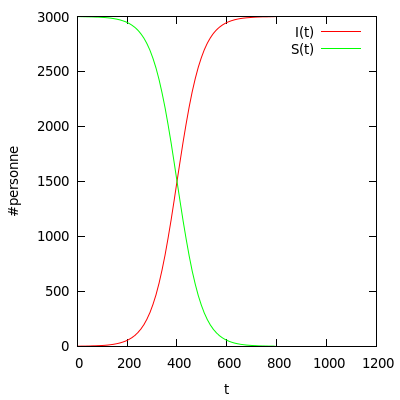
\includegraphics{Images/plotting_Q3_1.png} 
    %Il faudrait centrer l'image
    \caption{évolution de la population en fonction du temps}
    \label{fig:Q3.1}
\end{figure}

On peut remarquer sur la figure \ref{fig:Q3.1} que la fonction \( I \) converge rapidement vers son maximum. Cela via de la convergence
rapide de l'exponentielle décroissante vers sa limite. Ainsi, en environ 700 secondes, l'intégralité des machines vulnérables est
atteint. Il aura donc fallu moins de 12 minutes au ver pour contaminer l'ensemble du réseau pourtant composé de $3000$ machines. 
\end{homeworkSection}

%--------------------------------------------

\begin{homeworkSection}{Etude de l'influence du paramètre $\lambda$}
\begin{figure}[H]
    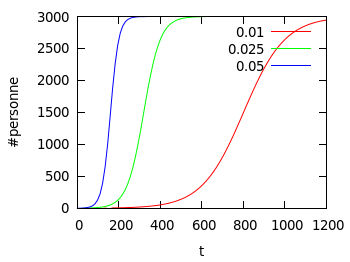
\includegraphics{Images/plotting_Q3_2.png}
    \caption{influence du paramètre $\lambda$}
    \label{fig:Q3.2}
\end{figure}

Dans l'équation différentielle présentée précédemment, le paramètre $\lambda$ correspond au nombre de contacts par machines par unité de temps. De ce fait, plus ce paramètre est élevé,
plus une machine peut atteindre d'autres machines entre deux pas de temps. Ainsi, si $\lambda$, augmente le nombre de machines
qu'une machine infectée peut contaminer augmente. Une illustration graphique de ce phénomène est visible sur la figure
\ref{fig:Q3.2}. On y voit en effet que la croissance de la courbe correspondant à $\lambda=0.05$ a une plus forte croissance que
les autres courbes (correspondant à $\lambda=0.025$ et $\lambda=0.01$).

\problemAnswer{ % Answer
    Avant de clôre cette partie sur le modèle déterministe, il est important de noter que les équations établies dans la première
partie ne traduisent pas la possibilité que deux machines infectées tente de contaminer la même machine.  En effet, l'équation:
\[
    \frac{dI(t)}{dt} = \lambda \cdot I(t) \cdot \frac{S(t)}{N}
\]
Implique que parmi toutes les machines contactées, la proportion de machines vulnérables ($\frac{S(t)}{N}$) sera infectée. Or il
est possible qu'une même machine soit atteinte par deux infectées distinctes. La solution de l'équation est donc un majorant de
$I$. En revanche, cette approximation est acceptable pour les grands réseaux (pendant le début de l'infection) où il est peu probable que deux infectées initient
une communication avec une même machine saine de part l'effet de nombre. Toutefois, sur de petits réseaux, ces équations de font
pas nécessairement sens.
}
\end{homeworkSection}

%--------------------------------------------

\end{homeworkProblem}

%----------------------------------------------------------------------------------------
%	PROBLEM 4
%----------------------------------------------------------------------------------------

\begin{homeworkProblem}[\arabic{homeworkProblemCounter} Modèle stochastique] % Roman numerals
\begin{homeworkSection}{Caractéristiques d'un modèle stochastique}
Modèle stochastique : Un processus stochastique est la représentation de l’évolution discrète ou en temps continu d’une variable
aléatoire. Dans un modèle probabiliste, on s'intéresse à l'évolution de manière probabiliste du modèle.
Dans notre cas, l’espace est dénombrable, on a donc un processus discret. On s’intéresse ici à l’évolution de la variable nombre
de machines infectées en fonction du temps avec un pas de temps de 1 seconde. On s'intéresse à la probabilité à un instant donné,
de pouvoir infecter une machine saine.  Une approche déterministe n'aurait pas été préférable, car l'évolution de l'infection
dépend de la probabilité à infecter une nouvelle machine au cours du temps. Dans l'article, nous avons l'étude de l'évolution de
l'infection selon 3 scénarios, dont deux possèdent un sous-réseau intermédiaire(la partie J du réseau). Or un modèle déterministe
ne pourrait prendre en compte correctement la probabilité de l'infection de la passerelle (gateway) entre les deux sous-réseaux(I
et K) ni la manière aléatoire de choisir les adresses à tester pour l'infection éventuelle.


De ce fait, une approche déterministe ne pourrait capturer les caractéristiques du phénomène étudié dans cet article. Elle telle
approche, donnerait en effet les mêmes résultats pour les trois scénarios, (Car étant par essence déterministe, elle ne peut
saisir le côté aléatoire du phénomène). Ainsi, l'auteur de pourrait conclure sur l'impact de la topologie d'un réseau sur la
propagation du vers.
\end{homeworkSection}
\end{homeworkProblem}

\begin{homeworkProblem}[\arabic{homeworkProblemCounter} Performance et optimisation] % Roman numerals
\begin{homeworkSection}{Application du concept du double-tétraèdre}
En nous situant dans un contexte d'optimisation, toujours en référant à l'article, nous pouvons situer notre double-tétraèdre dans un contexte d'optimisation.
Il faut prendre en compte les différentes stratégies possibles pour éviter l'infection et la propagation des vers au niveau de
l'attaqué.  L'attaquant quant à lui va chercher à infecter le plus grand nombre de machines, et le plus vite possible.

\begin{figure}[H]
    
\includegraphics{Images/doubleTetraedre.png}
    \caption{concept du double tétraèdre appliqué à l'article}
    \label{fig:Q5.1}
\end{figure}
%Pour Alex: J'ai rajouté deux trois trucs, dis moi si tu es d'accord :)
Les aspects du tétraèdre qui sont fixes sont :
L'environnement externe sur lequel nous ne pouvons pas agir. C'est-à-dire les facteurs extérieurs dont qui ne sont pas modifiables
ni par l'attaqué ni par l'attaquant. %Il faut voir précisément ce que l'on considère comme facteurs environnementaux 
Dans le cas présent, un premer élément serait le réseau externe: aucun des deux partis n'a de contrôle sur l'acheminement des
paquets. On peut également ajouter certains éléments de l'environnement interne: les ordinateurs du sous-réseaux. En effet, l'article de s'intéresse que à
l'effet de la topologie du réseau sur la propagation du vers. Ainsi, l'idée de modifier les ordinateurs afin de les protéger est
hors champ. Par exemple, l'idée de fermer les ports non-indispensables est pertinente, mais ne rentre pas dans le cadre de cet article.  
De plus, il semble naturel, dans le cadre de cet article, de supposer que l'attaquant ne peut altérer les ordinateurs afin de les rendre vulnérables à
l'infection. (Même si, dans le cadre général, quand on fait une analyse de risque, il faut considérer le cas d'une attaque
physique). On peut donc ajouter ces derniers à l'environnement.
\newline

Les aspects du tétraèdres qui sont modifiés sont :
\begin{itemize}
	\item Au niveau de l'attaqué, on va modifier les aspects de design et d'opération du réseau et des machines :
La topologie du réseau peut être modifié de telle sorte à ralentir la propagation d'une éventuelle infection. La mise en place de
logiciels appropriés comme des anti-virus peuvent permettre la diminution du nombre de machines infectées. La diversité des OS
peuvent aussi ralentir la propagation. %Pour Alex: Tu es sûr que l'ajout d'un anti virus rentre dans le cadre de l'article?
	\item Au niveau de l'attaquant, on va modifier les aspects de design et d'opération du ver : Les caractéristiques du ver
            de telle sorte à ce qu'il se propage plus vite, qu'il soit moins rapidement détectable et tout cela pour chercher
            l'augmentation du nombre de machines infectées. (Comme exemple de modification de design, on peut considérer l'ajout
            d'une hitlist ou encore une meilleure répartition des adresses à attaquer entre les vers)(Ces concepts sont introduits
            dans l'article \textit{how to own the inernet on your spare time}, l'une des références de \textit{Optimizing network against
            malware}).
	\end{itemize}
\end{homeworkSection}
\begin{homeworkSection}{Compléments d'études}
Les autres aspects/méthodes qui pourraient être étudiés dans le cadre d'un problème d'optimisation où l'objectif est de limiter la vitesse de propagation d'un logiciel malveillant dans un réseau sont :
\begin{itemize}
	\item Mise en place d'un IDS pour détecter les trafics étranges sur le réseau
	\item Mise en place d'anti-virus sur les machines
	\item Fermer les ports inutiles sur les machines, ne garder que les ports nécessaires actifs
	\item Essayer de détecter le ver à l'infection, par exemple si l'infection se fait par mail, le vers peut être détecter
            par un scan du mail %Pour Alex: C'est pas redondant avec l'ajout d'un anti virus?
        \item Utilisation de différents systèmes d'exploitation et de logiciels (afin que les machines ne soient pas toutes
            vulnérables aux mêmes attaques)
	\item Éducation des utilisateurs sur les comportements à risque. 
	\item Mise à jour régulière des logiciels pour combler des failles potentielles
	\item Aspect logiciel, aspect matériel %Pour Alex: C'est pas un peu trop vaque? ou tu penses que ça passe?
\end{itemize}
\end{homeworkSection}
\begin{homeworkSection}{La diversité dans un réseau informatique}
On peut appliquer le concept de diversité au sein d'un réseau informatique en utilisant des systèmes d'exploitation différents(Windows, Linus, Mac OS) selon le rôle de la machine dans le réseau. 
Cette diversité prendrait la forme d'une diversité au niveau logiciel(client de mail différent, système d'exploitation, ...), les
failles de sécurité ne seront plus les mêmes. Il pourrait aussi y avoir une diversité au niveau du matériel utilisé pour avoir des
drivers différents, et éventuellement limiter le nombre de machines pouvant être infectées par une faille d'un driver. L'idée
serait donc d'avoir des machines les plus différentes possibles. En effet, les systèmes d'exploitations différents ne fonctionnent
pas de la même façon, les logiciels et les programmes ne se lancent pas de la même manière, les failles ne sont donc pas les
mêmes, ce qui obligerait l'attaquant à créer un ver beaucoup plus complexe qui pourrait être capable de les infecter. 
%Pour Alex: Dis moi si tu valides la suite :)
On peut également envisager une diversité des utilisateurs, au sens où il y aurait des utilisateurs à faibles privilèges et des
administrateurs. Les utilisateurs à faibles privilèges ne pourraient lancer que certains programmes, mais ne pourraient pas lancer
d'installation sans intervention de l'administrateur. Ainsi, il faudrait que le ver infecte un administrateur afin de pouvoir se
propager efficacement. (On supposerait que les administrateurs sont moins nombreux et mieux formés que les autres).
\end{homeworkSection}
\end{homeworkProblem}
%----------------------------------------------------------------------------------------

\end{document}
